%\documentclass[journal]{IEEEtran}
%\documentclass[journal,11pt,draftclsnofoot,twocolumn]{IEEEtran}
%\documentclass[journal,11pt,draftclsnofoot,onecolumn]{IEEEtran}

\documentclass[12pt, draftclsnofoot, onecolumn]{IEEEtran}
\usepackage{cite}
\usepackage{amsmath,amssymb,amsfonts}
\usepackage{algorithm}
\usepackage{algorithmic}
\usepackage{graphicx}
\usepackage{textcomp}
\usepackage{xcolor}
\usepackage{color}
\usepackage{bm}
\usepackage{subfigure} 
\usepackage{booktabs}
\usepackage{cleveref}
%\documentclass[12pt, draftclsnofoot, onecolumn]{IEEEtran}
%
% If IEEEtran.cls has not been installed into the LaTeX system files,
% manually specify the path to it like:
% \documentclass[journal]{../sty/IEEEtran}

% *** GRAPHICS RELATED PACKAGES ***
%
\ifCLASSINFOpdf
  % \usepackage[pdftex]{graphicx}
  % declare the path(s) where your graphic files are
  % \graphicspath{{../pdf/}{../jpeg/}}
  % and their extensions so you won't have to specify these with
  % every instance of \includegraphics
  % \DeclareGraphicsExtensions{.pdf,.jpeg,.png}
\else
  % or other class option (dvipsone, dvipdf, if not using dvips). graphicx
  % will default to the driver specified in the system graphics.cfg if no
  % driver is specified.
  % \usepackage[dvips]{graphicx}
  % declare the path(s) where your graphic files are
  % \graphicspath{{../eps/}}
  % and their extensions so you won't have to specify these with
  % every instance of \includegraphics
  % \DeclareGraphicsExtensions{.eps}
\fi

\hyphenation{op-tical net-works semi-conduc-tor}


\begin{document}
%
% paper title
% Titles are generally capitalized except for words such as a, an, and, as,
% at, but, by, for, in, nor, of, on, or, the, to and up, which are usually
% not capitalized unless they are the first or last word of the title.
% Linebreaks \\ can be used within to get better formatting as desired.
% Do not put math or special symbols in the title.
\title{Learning-based Robust and Secure Transmission for Reconfigurable Intelligent Surface Aided Millimeter Wave UAV Communications}
%
%
% author names and IEEE memberships
% note positions of commas and nonbreaking spaces ( ~ ) LaTeX will not break
% a structure at a ~ so this keeps an author's name from being broken across
% two lines.
% use \thanks{} to gain access to the first footnote area
% a separate \thanks must be used for each paragraph as LaTeX2e's \thanks
% was not built to handle multiple paragraphs
%

\author{Xufeng~Guo,~Yuanbin Chen~and~Ying~Wang,~\IEEEmembership{Member,~IEEE}% <-this % stops a space
	
\thanks{	
	\textit{Corresponding author: Ying Wang.}
	
	X. Guo, Y. Chen, and Y. Wang are with the State Key Laboratory of Networking and Switching Technology, Beijing University of Posts and Telecommunications, Beijing, China 100876 (e-mail:brook1711@bupt.edu.cn; chen\_yuanbin@163.com; wangying@bupt.edu.cn).% <-this % stops a space
%\thanks{Manuscript received April 19, 2005; revised August 26, 2015.}
}}


% make the title area
\maketitle

% As a general rule, do not put math, special symbols or citations
% in the abstract or keywords.
\begin{abstract}
In this letter, we study the robust and secure transmission in the millimeter-wave (mmWave) unmanned aerial vehicle (UAV) communications assisted by the reconfigurable intelligent surface (RIS) under imperfect channel state information (CSI). Specifically, the active beamforming of the UAV, the coefficients of the RIS elements and the UAV trajectory are jointly designed to maximize the sum secrecy rate of all legitimate users in the presence of multiple eavesdroppers. However, the formulated problem is intractable mainly due to the complex constraints resulted from the intricate coupled variables and the time-related issue caused by outdated CSI.  To tackle these difficulties, by leveraging the deep deterministic policy gradient (DDPG) framework, a novel and effective twin-DDPG deep reinforcement learning (TDDRL) algorithm is proposed. Simulation results demonstrate the effectiveness and robustness of the proposed algorithm, and the RIS can significantly improve the sum secrecy rate.
\end{abstract}

% Note that keywords are not normally used for peerreview papers.
\begin{IEEEkeywords}
Deep reinforcement learnig, reconfigurable intelligent surface, physical layer security, unmanned aerial vehicle, millimeter-wave communications.
\end{IEEEkeywords}

% For peer review papers, you can put extra information on the cover
% page as needed:
% \ifCLASSOPTIONpeerreview
% \begin{center} \bfseries EDICS Category: 3-BBND \end{center}
% \fi
%
% For peerreview papers, this IEEEtran command inserts a page break and
% creates the second title. It will be ignored for other modes.
\IEEEpeerreviewmaketitle



\section{Introduction}

Millimeter-wave (mmWave) communications with multi-gigahertz bandwidth availability boost much higher capacity and transmission rate than conventional sub-6GHz communications. Unmanned aerial vehicles (UAVs), which are featured by their high mobility and flexible deployment, are promising candidates to compensate most of the deficiencies of mmWave signals, preserve its advantages, and provide more opportunities \cite{UAVMMWAVE-2}. However, the mmWave signals transmitted by UAVs are prone to deteriorate due to their high sensitivity to the presence of spatial blockages, especially in the complex propagation environment (such as in urban areas), which thus degrades the reliability of the communication links. In addition, broadcasting and superposition, as two basic properties of the wireless communication, make wireless transmissions inherently susceptible to security breaches \cite{RIS-20}. Hence, secure transmission is a pivotal issue in UAV communication systems which attracted extensive interest of researches \cite{RISUAV-1,RISUAV-9}.

Recently, the reconfigurable intelligent surface (RIS) composed of a large number of passive reflecting elements has become a revolutionary technology to achieve high spectral and energy efficiency in a cost-effective way \cite{RIS-101}. By appropriately tuning the reflection coefficients, the reflected signal can be enhanced or weakened at different receivers. Since the RIS has significant passive beamforming gain, it can be incorporated into the mmWave UAV communication system to generate virtual line-of-sight (LoS) links, thereby achieving directional signal enhancement, expanding coverage area and reducing radio frequency (RF) chains \cite{RISUAV-7}.

A crucial issue in the RIS-aided mmWave UAV communication system is to jointly design the active and passive beamforming and the UAV trajectory to guarantee the secure transmission. However, unlike the general RIS-aided wireless communication model, the UAV mobility-induced variation of the angles of arrival/departure (AoAs/AoDs) render the channel gains of all links (including direct links and cascaded links) to be optimization variables that need to be well-designed. Such variables are intricately coupled together with the active and passive beamforming matrix, which greatly increases the difficulty of the design. To circumvent this issue, several researches have been investigated in \cite{RIS-3,RISUAV-1,RISUAV-5,RISUAV-6,RISUAV-9}, some of which, in particular, leverage alternating optimization (AO) method to tackle the coupled variables \cite{RIS-3,RISUAV-1,RISUAV-5,RISUAV-9}. In \cite{RISUAV-6}, a deep reinforcement learning approach is utilized to jointly optimize the passive beamforming and the UAV trajectory, in which, however, the active beamforming is not considered in this approach. Nevertheless, all these existing works~\cite{RIS-3,RISUAV-1,RISUAV-5,RISUAV-6} are based on the assumption of the perfect channel state information (CSI), which weakens the versatility and practicality of the model. Furthermore, the UAV mobility-induced outdated CSI should also be taken into account. 

The deep reinforcement learning (DRL) is an efficient approach to jointly design the active and passive beamforming, and the UAV trajectory, due to its good generalization, low complexity, and high accuracy characteristics. The motivation of utilizing DRL approach is mainly for two reasons: i) it is fairly difficult to tackle the intricately coupled variables in the RIS-aided UAV system, and even the widely applicable AO method cannot solve this problem well, especially for the multi-user system. ii) the UAV mobility-induced CSI is easily outdate, and there is in general no effective method to solve such a time-related issue.


In this letter, motivated by these considerations, we investigate the secure transmission problem in the RIS-aided mmWave UAV communication system. The active beamforming at the UAV, the passive beamforming at the RIS and the UAV trajectory are jointly designed by explicitly taking into account imperfect CSI. First, to enhance the robustness of the considered system, we study a secrecy rate maximization problem subject to the secrecy outage probability resulted from the statistical CSI error model. Moreover, to solve this problem, a novel twin-deep deterministic policy gradien (DDPG) deep reinforcement learning (TDDRL) algorithm is proposed. More specifically, the first network is utilized to provide policy for the active and passive beamforming while the UAV trajectory is coordinated by the second network. Finally, The obtained simulation results demonstrate the effectiveness and the performance benefits of the proposed TDDRL algorithm.

\begin{figure}[t]
	%	Requires \usepackage{graphicx}
	\centering
	
\includegraphics[width=0.7\linewidth]{./plot/eps/system_with_H.eps}% 1\linewidth
	\caption{RIS-aided Milimeter Wave UAV Communications.}  %\label{fig}
\end{figure}

\section{System Model and Problem Formulation}

\subsection{System Model}
In this letter, we consider an RIS-aided mmWave UAV communication system where an RIS is exploited to assist the secure downlinks from the UAV to $K$ single-antenna legitimate users in the presence of $P$ single-antenna eavesdroppers. Specifically, the UAV is equipped with an $A$-element uniform linear array (ULA), and the RIS has a uniform planar array (UPA) with $M{\rm =}m^2$ passive reflecting elements ($m$ is an integer). The set of the legitimate users and the eavesdroppers are denoted by ${\cal K}{\rm =}\{ 1,2,...,K \}$, ${\cal P}{\rm =}\{1,2,...,P \}$, respectively. As shown in Fig.1, all entities are placed in the three dimensional (3D) Cartesian coordinate system. The RIS is fixed at ${\bm{w}}_{R}{\rm{ = }}(x_R,y_R,z_R)^T$. We assume that the UAV flies at a fixed altitude in a finite time span which is divided into $N$ time slots, i.e., $T{\rm{ = }}N\delta_n$, where $\delta_n$ is the time slot. Then the coordinate of the UAV and the coordinates of the legitimate users and eavesdroppers at the $n$-th time slot are denoted by ${\bm{q}}[n]{\rm{ = }}(x_U[n],y_U[n],H_{U})^T$ and ${\bm{w}}_{i}{\rm{ = }}(x_i[n],y_i[n],z_i[n])^T,\forall i \in {\cal K}\cup{\cal P}$, respectively. The location information at the $n$-th time slot is defined as ${\bm W}{\rm \triangleq}\{{\bm q}[n]\}\cup \{{\bm w}_i[n]|\forall i \in {\cal K}\cup {\cal P}\}$. The UAV is subject to the following mobility constraints:

\begin{subequations}\label{mobility-1}
	\begin{gather}
  \|\bm{q}[n+1]-\bm{q}[n] \|^2 \leq D_{max}^2 , n=1, \ldots, N-1,\\
  \left\lvert x[n] \right\rvert ,\left\lvert y[n] \right\rvert  \leq B , n=1, \ldots, N,\\
  \bm{q}[0] \equiv (0,0,H_{U}), n=1, \ldots, N-1,
	\end{gather}
\end{subequations} 
where $D_{max}$ is the maximum moving distance at each time slot, and $B$ is the moving boundary of the UAV.

Let ${\bm{h}}_{U,k}\rm{\in} \mathbb{C}^{\emph{A}\times 1},$ $\bm{h}_{U,p} \rm{\in} \mathbb{C}^{\emph{A}\times 1},$ $ \bm{h}_{R,k} \rm{\in} \mathbb{C}^{\emph{M}\times 1},$ $\bm{h}_{R,p} \rm{\in} \mathbb{C}^{\emph{M}\times 1},$ 
$\bm{H}_{UR} \rm{\in} \mathbb{C}^{\emph{M}\times \emph{A}}$ be the channel gains from the UAV to $k$-th user, the UAV to the $p$-th eavesdropper, the RIS to the $k$-th user, the RIS to the $p$-th eavesdropper, the UAV to the RIS links, respectively. All the channels are modeled according to 3D SalehValenzuela channel model~\cite{mmwave-1} which has been widely used to characterize the mmWave channels:

\begin{subequations}\label{channel-1}
	\begin{align}
  &{\bm{h}}_{U,i}=\sqrt{\frac{1}{L_{UK}}} \sum_{l = 1}^{L_{UK}} g^{u}_{i,l}{\mathbf{a }}_{L}  \left(\vartheta_{i,l}^{AoD}\right),\forall i \in {\cal K}\cup {\cal P},\\
  &{\bm{h}}_{R,i}=\sqrt{\frac{1}{L_{RK}}} \sum_{l = 1}^{L_{RK}} g^{r}_{i,l}{\mathbf{a }}_{P}  \left(\vartheta_{i,l}^{AoD}, \varphi_{i,l}^{AoD}\right),\forall i \in {\cal K}\cup {\cal P},\\
  &{\bm{h}}_{UR}=\sqrt{\frac{1}{L_{RK}}} \sum_{l = 1}^{L_{RK}} g^{ur}_{l}{\mathbf{a }}_{P}  \left(\vartheta_{l}^{AoA},\varphi_{l}^{AoA}\right){\mathbf{a }}_{L}  \left(\vartheta_{l}^{AoD}\right)^H .
  \end{align}
\end{subequations}

\noindent In~(\ref{channel-1}), the large-scale fading coefficients defined by  $g \in \{g^u_{i,l},g^{r}_{i,l},g^{ur}_{l}\}$ follow a complex Gaussian distribution as ${\cal CN}(0, 10^{\frac{PL}{10}})$, where $\text{PL(dB)} {\rm} {\rm =}  {\rm -}C_0{\rm -10 \alpha }{\rm log}_{10}({D}){\rm -}{\rm PL}_s$, $C_0$ is the path loss at a reference distance of one meter, $\text{D}\ \text{(meters)}$ is the link distance, $\alpha$ denotes the path-loss exponent, and $\text{PL}_s {\rm \sim} {\cal CN}(0, \sigma_s^2)$ is the shadow fading component. The steering vector of the ULA is denoted by $\mathbf{a}_{L}(\vartheta){\rm =}\left[1, e^{j \frac{2 \pi}{\lambda c} d \sin (\vartheta)}, \ldots, e^{j \frac{2 \pi}{\lambda c} d(A-1) \sin (\vartheta)}\right]^{H}$, where $\vartheta$ stands for the azimuth AoD $\vartheta_{i,l}^{AoD}$ and $ \vartheta_{l}^{AoD}$, $d$ is the antenna inter-spacing, and $\lambda_c$ is the carrier wavelength. The steering vector of the UPA is denoted by $\mathbf{a}_{P}(\vartheta, \varphi){\rm =}\left[1, \ldots, e^{j \frac{2 \pi}{\lambda c} d(p \sin (\vartheta) \sin (\varphi)+q \cos (\vartheta) \sin (\varphi))}, \ldots\right]^{H}$, where $0\leq {p,q}\leq m-1$, and $\vartheta(\varphi)$ is the azimuth(elevation) AoD $\vartheta_{i,l}^{AoD}$($\varphi_{i,l}^{AoD}$) and the AoA $\vartheta_{l}^{AoA}(\varphi_{l}^{AoA})$.

The cascaded channel from the UAV to the $i$-th user or the eavesdropper can be written as $ \bm{H}_{C,i}{\rm =}\text{diag}(\bm{h}_{R,i}^H)\bm{h}_{UR},\forall i \in {\cal K}\cup {\cal P}$. The passive beamforming matrix of the RIS is denoted by ${\bm{\Theta }} {\rm =} {\rm{diag}}\left( {{\beta _1}{e^{j{\theta _1}}},{\beta _2}{e^{j{\theta _2}}},...,{\beta _M}{e^{j{\theta _M}}}} \right)$, where ${\theta _m} \in \left[ {\left. {0,2\pi } \right)} \right.$, ${\beta _m} \in \left[ {0,1} \right], m {\rm =}\{1,2,\cdots ,M\}$ represent the phase shift and amplitude reflection coefficients of the $m$-th RIS reflection element, respectively. The amplitude reflection coefficients are set to one, i.e., ${\beta _m} {\rm =}1 $ to simplify the problem and maximize the power of the reflecting signal~\cite{secure-1}. Let ${\bm H}_{C}\triangleq \{{\bm h}_{U,i}^{H}+\bm{\Psi}^{H}\bm{H}_{C,i} |\forall i \in {\cal K}\cup {\cal P} \}$ denote the combined channel gains between the UAV and all receivers. Let $\bm{\Psi}{\rm =}\text{vec}(\bm{\Theta}) $ denote the vectorized passive beamforming vector. Thus, the received signal at the $i$-th user or eavesdropper from the UAV can be formulated as
\begin{equation}\label{received-1}
  y_i=({\bm{h}}_{U,i}^H+{\bm{\Psi}^{H}\bm{H}}_{C,i}){\bm{G}}{\bm{s}}+ {{n}_{i}},\forall i\in {\cal K}\cup{\cal P},
\end{equation}
\noindent where $ {\bm s}\in {\mathbb C}^{K\times 1}$ with $E[|s_k|^2]{\rm =}1 $ and $ {\bm{G}} \in \mathbb{C}^{{A} \times {K}}$ represents the transmitted symbol and the beamforming matrix at the UAV, and it is assumed that $ n_i \sim {\cal N}(0,\sigma_n),\forall i \in {\cal K}\cup {\cal P}$. Let $\bm{g}_k$ be the $k$-th column of the beamforming matrix $\bm{G}$. Then, the achievable rate of the $k$-th user is given by
\begin{equation}\label{unsecure-1}
  R_k^u = {\rm log}_2\left(1+\frac{|(\bm{h}_{U, k}^{H}+{\bm \Psi}^{H} \bm{H}_{C, k})\bm{g}_k|^2}{\sum_{k^{'} \in {\cal K}\backslash k}  | {}\bm{h}_{U, k}^{H}+{\bm \Psi}^{H} \bm{H}_{C, k})\bm{g}_{k^{'}} |^2+n_k^2}\right).
\end{equation}

If the $p$-th eavesdropper aims to eavesdrop the signal of the $k$-th user, its achievable rate can be denoted by 
\begin{equation}\label{eavesdrop-1}
  R_{p,k}^e = {\rm log}_2\left(1+\frac{|(\bm{h}_{U, p}^{H}+{\bm \Psi}^{H} \bm{H}_{C, p})\bm{g}_k|^2}{\sum_{k^{'} \in {\cal K}\backslash k}  | {}\bm{h}_{U, p}^{H}+{\bm \Psi}^{H} \bm{H}_{C, p})\bm{g}_{k^{'}} |^2+n_p^2}\right).
\end{equation}

The achievable individual secrecy rate from the UAV to the $k$-th user~\cite{secure-1} can be expressed by
\begin{equation}\label{secure}
  R_{k}^{\mathrm{sec}}=\left[R_{k}^{\mathrm{u}}-\max _{\forall p} R_{p, k}^{\mathrm{e}}\right]^{+}, 
\end{equation}
where $[z]^{+}=\max (0, z)$.

In the practical system, the perfect CSI is not available at the UAV due to the transmission delay and processing delay, as well as the mobility of the UAV and the users. The CSI may be stale at the time when the UAV transmits the data stream to the RIS and the users, which results in an inevitable performance loss once this outdated CSI is employed for transmission. Thus, the outdated CSI should be explicitly considered in the system design.


%It is worth noting that the outdated CSI will lead to substantial performance loss in practical systems. According to~\cite{CSI-error-1}, the outdated CSI can be expressed as statistical CSI error model. 

Let $T_d$ be the delay between the outdated CSI and the real-time CSI. The relation between the outdated channel vector $\bm{h}(t)$ and the real-time channel vector $\bm{h}(t+T_d)$ can be expressed as~\cite{CSI-error-2}

\begin{equation}\label{CSI-error-1}
  \bm{h}\left(t+T_{\text {d }}\right)=\varrho \tilde{\bm{h}}(t)+\sqrt{1-\varrho^{2}}\Delta \bm{h},
\end{equation}
where $\Delta {\bm{h}}$ is the error term that is independent identically distributed (i.i.d) with $\bm{h}\left(t+T_{\text {d }}\right)$ and $\tilde{\bm{h}}(t)$, $\varrho $ is the autocorrelation function of the channel gain $\bm{h}(t)$, given by the zeroth-order Bessel function of the first kind as
%\begin{equation}\label{CSI-autocorrelation}
  $ \varrho=J_{0}\left(2 \pi f_{D} T_{\mathrm{d}}\right) $,
%\end{equation}
where $f_D$ is the Doppler spread which is expressed as $f_{D}=v f_{c} / c$, and $v$, $f_c$, $c$ represent the velocity of the transceivers, the carrier frequency and the speed of light, respectively. 

Note that due to the stochastic nature of the error $\Delta \tilde{\bm{h}}$, the error model in (\ref{CSI-error-1}) belongs to statistical error model in essence \cite{CSI-error-1,CSI-error-2}. The autocorrelation function $ \varrho $ bridges the real-time $ \bm{h}\left(t+T_{\text {d }}\right) $ with the estimated $\tilde{\bm{h}}(t)$ that is easily outdated. The actual CSI $ \bm{h} \triangleq \{ \bm{h}_{\mathrm{U}, i},\bm{h}_{\mathrm{R}, i},\bm{h}_{\mathrm{UR}}, \forall i \in \mathcal{K} \cup \mathcal{P}\} $ can be expressed as the form in (\ref{CSI-error-1}). Furthermore, the system can only access to the estimated CSI $ {\tilde{\bm{h}}} \triangleq \{ \tilde{\bm{h}}_{\mathrm{U}, i},\tilde{\bm{h}}_{\mathrm{R}, i},\tilde{\bm{h}}_{\mathrm{UR}}, \forall i \in \mathcal{K} \cup \mathcal{P} \} $\footnote{We assume that the CSI can be obtained by adopting the channel estimation method in the RIS aided system, such as \cite{footnote}.  } that are outdated, and the actual CSI $ \bm{h} $ given by (\ref{CSI-error-1}) is employed to calculate achievable secrecy rate in (\ref{unsecure-1})-(\ref{secure}).

\subsection{Problem Formulation}

In this letter, we aim to maximize the sum secrecy rate $\sum_{k=1}^{K}  R_{k}^{\mathrm{sec}} $ by jointly optimizing the UAV's trajectory ${\bm{Q}} \triangleq\{{\bm q }[n], n {\rm =}{1,2,\cdots,N}\}$ and the active (passive) beamforming matrix $\bm{G}$($\bm{\Theta}$), which yields the following problem
\begin{subequations}\label{formulation}
  \begin{align}
    &\mathop {\max }\limits_{{\bm{Q}},{\bm{G}},{\bm{\Theta }}} \quad\sum\limits_{k \in {\cal K}} {{R_k^{\mathrm{sec}}}}\\
    s.t.\qquad &(\ref{mobility-1}),\\
    &\operatorname{Pr}\left\{{R_k^{\mathrm{sec}}} \geq R_{k}^{\mathrm{sec,th}}\right\} \geq 1-\rho_{k}, \forall k \in \mathcal{K},\\
    &\operatorname{Tr}\left(\bm{G} \bm{G}^{H}\right) \leq P_{\max },\\
    &{\theta _m} \in \left[ {\left. {0,2\pi } \right)} \right. , m = \{1,2,\cdots, M\},
  \end{align}
\end{subequations}
where the secrecy rate outage constraint in~(\ref{formulation}\rm{c}) guarantees that the probability that each legitimate user can successfully decode its message at a data rate of $ R_{k}^{\mathrm{sec,th}}$ is no less than $1-\rho_k$. Problem (\ref{formulation}) is intractable mainly for the non-convex constraints in (\ref{formulation}b), (\ref{formulation}c), and (\ref{formulation}e), the secrecy outage constraint without close-form expression, and the time varying CSI described in~(\ref{CSI-error-1}). There is in general no standard method to solve such a probability-constrained non-convex optimization. Next, a DRL-based approach is proposed to overcome these challenges effectively.
\begin{figure}[t]
	%	Requires \usepackage{graphicx}
	\centering
	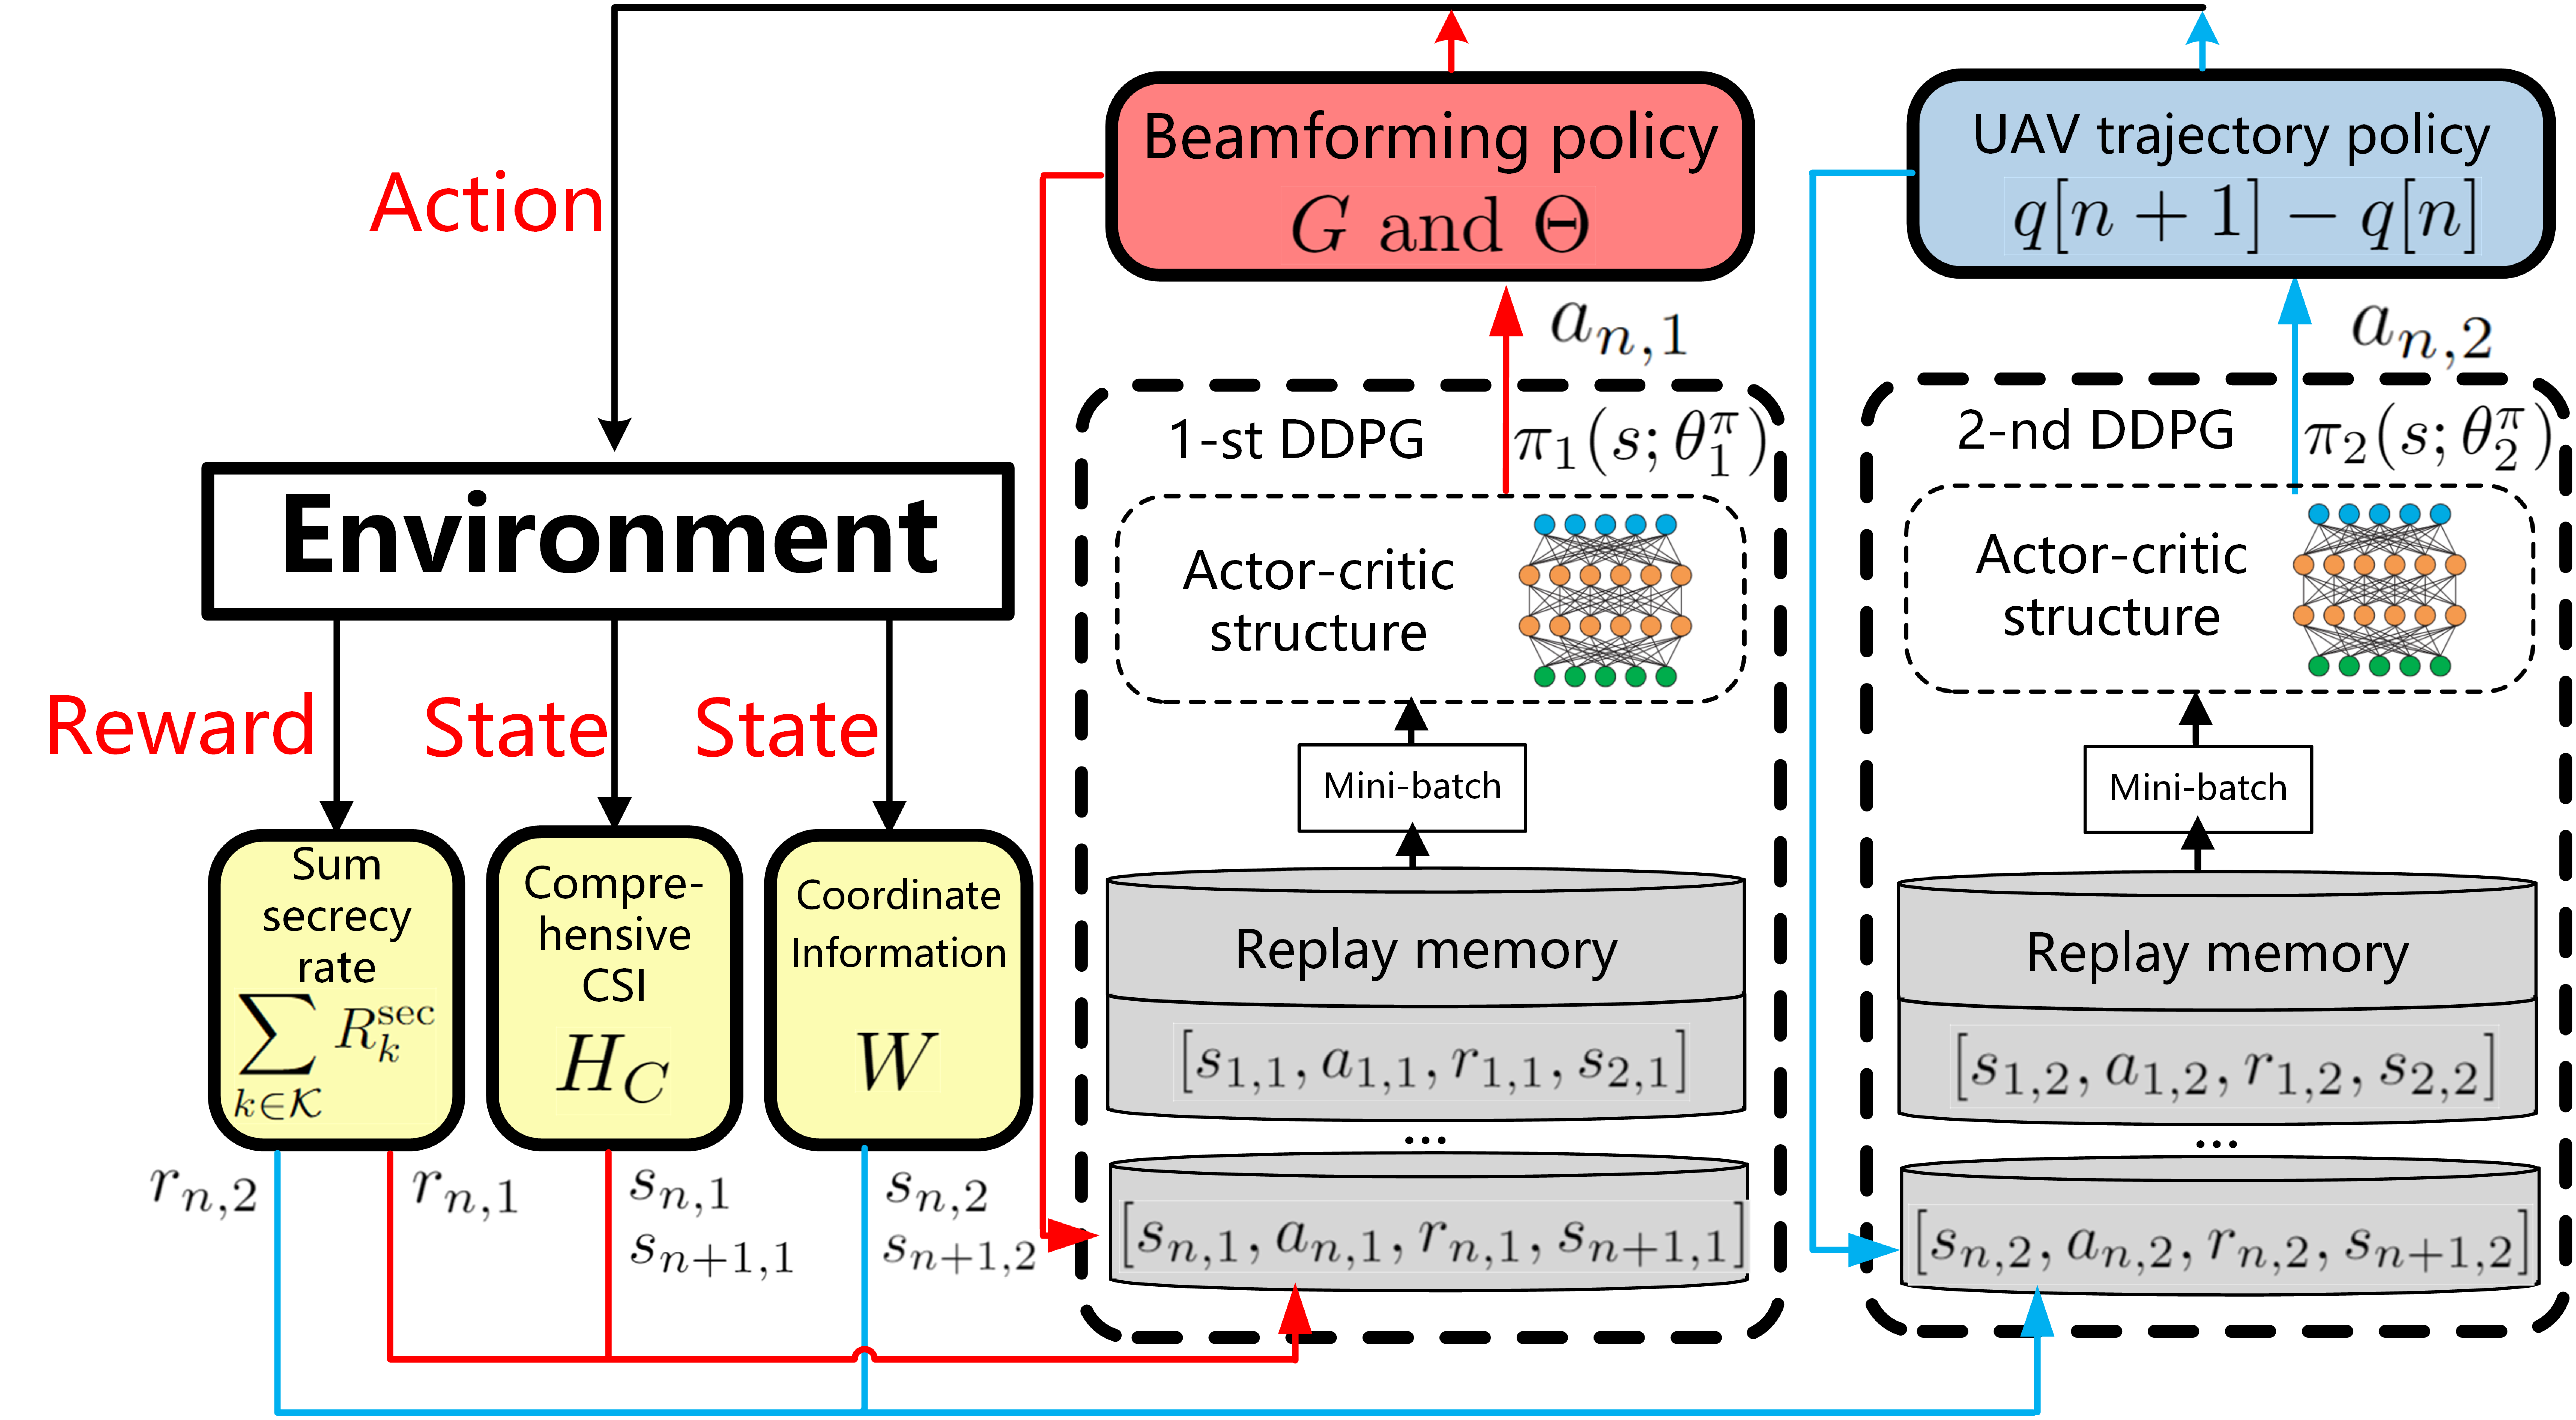
\includegraphics[width=0.8\linewidth]{./plot/eps/construction_v2.eps}% 1\linewidth
	\caption{Structure of the proposed TDDRL algorithm.}  \label{structure}
\end{figure}
\section{DRL-based Solution}
To solve problem~(\ref{formulation}), we propose a TDDRL algorithm, which is able to allow the agent to learn the policies of the beaforming and the trajectory without any prior knowledge of the system. Since the UAV trajectory ${\bm Q}$ is highly coupled with large amounts of CSI, it is difficult to optimize all the variables simultaneously, which may incur a poor convergence and performance. To tackle this issue, two DDPG networks are constructed to decouple these variables instead of employing a single agent in the conventional DRL-based network. In particular, as illustrated in Fig.2, the first network takes the CSI, i.e., ${\bm H}_{C}$ as the state to obtain the optimal $\bm{G} $ and $\bm{\Theta} $, the second network takes the coordinates of the UAV and all legitimate users and eavesdroppers as the state, i.e., ${\bm W} $ to obtain the UAV movement which consists of the flying distance $\mu[n]$ and direction $\psi[n]$ at the $n$-th time slot. Both networks share the same reward function. The design of the DRL-based solution are elabarated as follows.

\begin{algorithm}[t]
	\caption{TDDRL Algorithm}
	\begin{algorithmic}[1]
    \STATE {Initialize the actor and critic networks $\pi_1(s;{\bm \phi}^{\pi}_{1}) $, $Q_1(s,a;{\bm \phi}^{Q}_1)$, target actor and critic networks $\pi^{'}_{1}(s;{\bm \phi}^{\pi^{'}}_{1}) $, $Q^{'}_1(s,a;{\bm \phi}^{Q^{'}}_1)$ of the first DDPG network;}
    \STATE {Similarly, Initialize $\pi_2(s;{\bm \phi}^{\pi}_{2}) $, $Q_2(s,a;{\bm \phi}^{Q}_2)$, $\pi^{'}_{2}(s;{\bm \phi}^{\pi^{'}}_{2}) $, $Q^{'}_2(s,a;{\bm \phi}^{Q^{'}}_2)$ for the second DDPG network;}
    \FOR {Episode $n_{ep} = 1,2,...,N_{ep}$ of the second DDPG network}
      \STATE {Reset the positions of the UAV and all users;}
      
      \FOR {Step $n = 1,2,...,N_{step}$}
        \STATE{Observe ${\bm H}_C $ as $s_{n,1}$, and ${\bm W}$ as $s_{n,2}$;}
        \STATE{Select actions $a_{n,1},a_{n,2}$ with a gaussian action noise $n_{a}$ with variance $\sigma_a$ :
        
            $a_{n,1}=\pi_1(s;{\bm \phi}^{\pi}_{1}) +n_{a}$, 
            $a_{n,2}=\pi_2(s;{\bm \phi}^{\pi}_{2}) +n_{a}$
        }
        \STATE{Execute actions $a_{n,1},a_{n,2}$, receive an immediate reward $r_{n,1}{\rm =}r_{n,2}$ According to Eq.~(\ref{reward}) and receive new states $s_{n+1,1},s_{n+1,2}$ from the environment;}
        \STATE{Store the transitions $[s_{n,1},a_{n,1},r_{n,1},s_{n+1,1}]$ and $[s_{n,2},a_{n,2},r_{n,2},s_{n+1,2}]$ into the memory queues;}
        \STATE{Sample mini batchs to update ${\bm \phi}^{\pi}_i$, ${\bm \phi}^{Q}_i,i{\rm \in}\{1,2\}$;}
        \STATE{Update ${\bm \phi}^{\pi^{'}}_i$, ${\bm \phi}^{Q^{'}}_i,i{\rm \in}\{1,2\}$;}
      \ENDFOR
    \ENDFOR
	\end{algorithmic}
\end{algorithm}

\subsection{Active and Passive Beamforming}
Inspired by the work of~\cite{secure-1}, the first DDPG network is employed to learn the optimal policy in terms of the beamforming matrix $\bm{G}$ of the UAV and reflecting beamforming matrix $\bm{\Theta}$ of the RIS by interacting with the whole system. Each episode is defined as a time span $T$, where each step is defined as a time slot $\delta_n$. In order to maximize the sum secrecy rate, the state $s_{n,1}$, the action $a_{n,1}$ and the reward $r_{n,1}$ of the first network at the $n$-th time slot are defined as follows:
\begin{itemize}
  \item [1)] 
  \textbf{State} $s_{n,1}$: the state of the first agent in the $n$-th time slot contains the estimated comprehensive CSI from the UAV to all legitimate users and eavesdroppers, i.e., ${\bm H}_{C}$.
  \item [2)]
  \textbf{Action} $a_{n,1}$: we define the the passive beamforming matrix ${\bm \Theta}$ and the active beamforming matrix ${\bm G }$ as action. It is worth noting that ${\bm G} = Re\{ {\bm G} \} + Im\{ {\bm G} \}$ and ${\bm \Theta} = Re\{ {\bm \Theta} \} + Im\{ {\bm \Theta} \}$ are separated as real part and imaginary part to tackle with the real input problem.
  \item [3)]
  \textbf{Reward} $r_{n,1}$: the reward function is defined as:
  \begin{equation}\label{reward}
    r_{n,1}={\rm tanh}(\sum_{k=1}^{K}  R_{k}^{\mathrm{sec}}-c_1 p_{m}- c_2 p_{r}-c_3 p_{g}),
  \end{equation}
  where $p_{m}$, $p_{r}$ and $p_{g}$ are the penalties when the constraints~(\ref{formulation}\rm{b}),~(\ref{formulation}\rm{c}) and~(\ref{formulation}\rm{d}) are not satisfied, respectively. The coefficients $c_i,i{\rm \in}\{1,2,3\} $ are the weights for balancing the penalties and the sum secrecy rate. The value of the outage probabilities at each time step are estimated by 500 ${\bm H}_C$ samples generated according to the statistical CSI error model in~(\ref{CSI-error-1}). The hyperbolic tangent function $\text{tanh}(\cdot )$ is exploited to limit the reward in the range of $(-1,1)$ for a better convergence.
\end{itemize}
\subsection{UAV Trajectory}
The second DDPG network is exploited to simultaneously obtain the optimal movement ${\mu}[n]$ and $\psi[n]$ with ${\bm G}$ and $\bm{\Theta}$. The state $s_{n,2}$, the action $a_{n,2}$ and the reward $r_{n,2}$ of the second network at the $n$-th time slot are defined as follows:
\begin{itemize}
  \item [1)] 
  \textbf{State} $s_{n,2}$: as mentioned before, the UAV trajectory is highly coupled with the large amounts of CSI. Thus, we take only the location information ${\bm W}$ as the state of the second network to decouple the variables.
  \item [2)]
  \textbf{Action} $a_{n,2}$: the action contains the UAV's flying distance $\mu[n] $ and the direction $\psi[n] $. Then, the movement of the UAV at the $n$-th time slot can be expressed as:
    ${\bm q}[n+1]-{\bm{q}}[n]=\mu[n]({\rm cos}\psi[n] {\bm{e}}_x+ {\rm sin}\psi[n] {\bm{e}}_y)$, 
    where ${\bm{e}}_x$, ${\bm{e}}_y$ are the unit vector on the X-axis and the Y-axis. 
  \item [3)]
  \textbf{Reward} $r_{n,2}$: the same reward function in~(\ref{reward}) is employed, since both networks have the same objective to maximize the sum secrecy rate.
\end{itemize}
% 总结一下TDDRL的结构:采用上述的双DDPG结构,可以使两个网络分别优化主被动波束和UAV轨迹从而减少优化变量之间的耦合。随着训练过程的进行,第一个模型可以得出在相应CSI条件下的主被动波束策略,第二个模型可以根据模型中实体的位置信息得出UAV的最优轨迹策略。从而,得到优化的三方联合的结果    同时考虑主被动波束

As the training process turns to converge, the first network derives the optimal active and passive beamforming strategy, and the second network imparts the optimal trajectory. The shared reward function and environment information allow these two networks to coordinate with each other to learn a favorable policy. Thus, the beamforming matrix (${\bm G}$, ${\bm \Theta}$), and the UAV trajectory ${\bm Q}$ are achieved according to the proposed TDDRL algorithm. The overall algorithm for solving problem~(\ref{formulation}) is summarized in Algorithm 1. 
\subsection{Computational Complexity Analysis}
This subsection mainly discusses the computational complexity of the proposed TDDRL algorithm. In particular, let $L$ and $n_{i}$ denote the layers number of the deep neural network (DNN) exploited in the DDPG networks and the neurons number in the $i$-th layer, respectively. For the training mode, the computational complexity for a single DNN to both evaluate and update in a single step is ${\mathcal O}(N_{b}(\sum_{i=1}^{L-1} n_{i}n_{i+1})) $~\cite{secure-1}, where $N_{b}$ is the size of the mini-batch. Since the TDDRL algorithm is composed of finite number of DNNs, and it takes $N_{ep}*N_{step}$ steps to finish training, the total training computational complexity of the TDDRL algorithm is ${\mathcal O}(N_{ep}N_{step}N_{b}(\sum_{i=1}^{L-1} n_{i}n_{i+1})) $. For the working mode, the computational complexity in each step dramatically decreases to ${\mathcal O}(\sum_{i=1}^{L-1} n_{i}n_{i+1}) $ due to the absence of the training procedure.

\begin{table}[t]
  \centering
  \caption{Main Parameters.}
  \begin{tabular}{cc} 
  \toprule
  Parameter              & Value    \\ 
  \hline
  UAV antenna number    &${{A}}=4$        \\
  RIS reflecting element number &${ M}=16$       \\
  eavesdropper number    &${{P}} = 1$        \\
legitimate user number &${{K}} =2$        \\
  step number            & $N_{step}=100$      \\
  episode number         & $N_{ep}=100$      \\
  carrier frequency      &$f_c=28\ \text{GHz}$\\
  max transmission power            &$P_{max }= 30\ \text{dBm}$  \\
  noise power            &$\sigma_n= -114\ \text{dBm}$  \\
  path loss at one meter &$C_0=61\ \text{dB} $\\
  path loss factor\cite{parameters}       &    $\alpha_{ur}=2.2,\alpha_{u}=3.5,\alpha_{r}=2.8$      \\
  shadow   fading factor &${\sigma}_s = 3\ \text{dB} $     \\
  \bottomrule
  \end{tabular}
\end{table}

\section{Simulation Results}
In this section, numerical results are presented to evaluate the performance of the proposed TDDRL algorithm. For the first DDPG network, we deploy four fully-connected hidden layers with [800, 600, 512, 256] neurons in both actor and critic networks and the adaptive moment estimation optimizer is used to train the actor network with learning rate 0.0001 and the critic network with learning rate 0.001. The second network has the same structure as the first network, but with different number of four layers [400, 300, 256, 128]. The initial coordinates of the UAV and the fixed RIS are set as (0 m, 25 m, 50m) and (0 m, 50 m, 12.5 m), respectively. The eavesdropper is placed at (47 m, -4 m, 0 m). Furthermore, we model the movements of two legitimate users as uniform motion in a straight line as shown in Fig.\ref{trajectory}. More detailed parameters are shown in Table \uppercase\expandafter{\romannumeral1}.


Fig.\ref{trajectory} illustrates the optimized trajectory, which eventually converges as the learning procedure is over. It can be observed that the UAV tends to move away from the eavesdropper. Moreover, the UAV is inclined to chase and follow the midpoint of two legitimate users' positions, while keeping relatively close distance to the RIS. This implies the UAV trajectory is jointly optimized with the active and passive beamforming, and the proposed algorithm can adapt to dynamic conditions brought by the mobility of the users.



Fig.\ref{compare} plots the average sum secrecy rate versus training episodes, where the following benchmarks are used for comparison: 1) the proposed TDDRL algorithm under imperfect CSI; 2) the proposed TDDRL algorithm under perfect CSI; 3) jointly design ${\bm G}$, ${\bm \Theta}$ and ${\bm Q}$ with a single DDPG network; 4) jointly design ${\bm \Theta}$ and ${\bm Q}$ while using static ${\bm G}$; 5) using static ${\bm \Theta}$; 6) using static ${\bm Q}$. It is found that the TDDRL algorithm which jointly optimizes ${\bm G}$, ${\bm \Theta}$ and ${\bm Q}$ achieves the best performance under imperfect CSI. Compared with the single DDPG scheme, the TDDRL algorithm has a better convergence and performance by configuring the same learning rate and layer number. However, there exists the performance gap in terms of the secrecy rate obtained by the TDDRL algorithm between perfect and imperfect CSI. This is expected and substantiates the importance of the robust design in the actual system.


\begin{figure}[t]
  \centering
  \begin{minipage}[t]{0.48\textwidth}
    \centering
    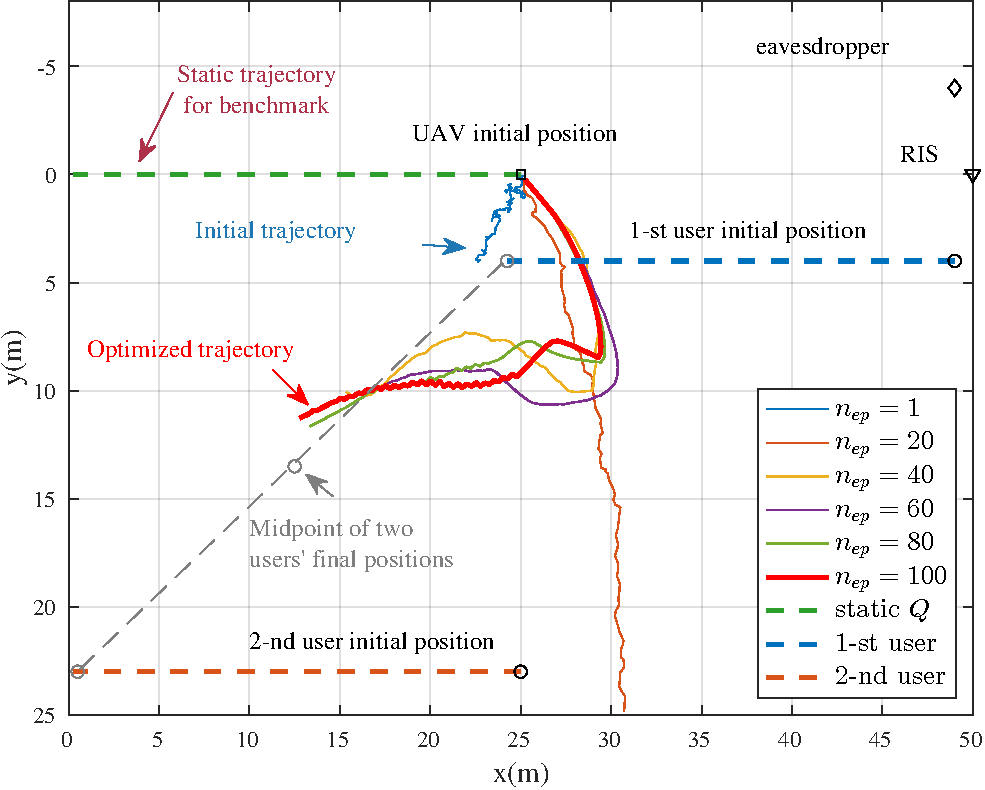
\includegraphics[width=0.8\linewidth]{./plot/trajectory/trajectory.pdf}% 1\linewidth
    \caption{Trajectory of the UAV optimized by the proposed TDDRL algorithm.}  %\label{fig}
    \label{trajectory}
  \end{minipage}
  \begin{minipage}[t]{0.48\textwidth}
    \centering
    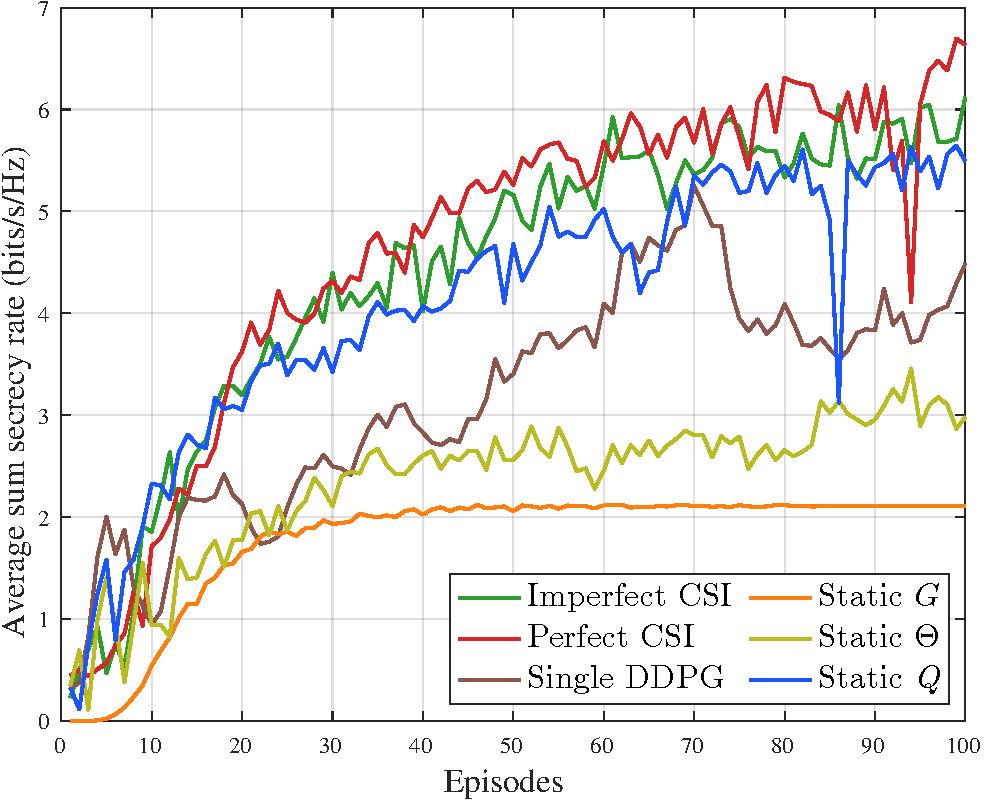
\includegraphics[width=0.8\linewidth]{./plot/compare/compare.pdf}% 1\linewidth
	  \caption{Accumulated reward performance versus episodes under different RIS elements number.}  %\label{fig}
  \label{compare}
  \end{minipage}
  
\end{figure}

\section{Conclusion}
In this letter, we investigate the robust and secure transmission for RIS-aided mmWave UAV communications. To maximize the sum secrecy rate of all legitimate users, we propose a TDDRL algorithm to effectively tackle the concerned issues. Simulation results validate that by jointly optimizing UAV trajectory and active (passive) beamforming, a better performance can be achieved compared with several benchmarks.





% if have a single appendix:
%\appendix[Proof of the Zonklar Equations]
% or
%\appendix  % for no appendix heading
% do not use \section anymore after \appendix, only \section*
% is possibly needed

% use appendices with more than one appendix
% then use \section to start each appendix
% you must declare a \section before using any
% \subsection or using \label (\appendices by itself
% starts a section numbered zero.)
%


%\appendices
%\section{Proof of the First Zonklar Equation}
%Appendix one text goes here.

% you can choose not to have a title for an appendix
% if you want by leaving the argument blank
%\section{}
%Appendix two text goes here.


% use section* for acknowledgment
%\section*{Acknowledgment}


%The authors would like to thank...


% Can use something like this to put references on a page
% by themselves when using endfloat and the captionsoff option.
%\ifCLASSOPTIONcaptionsoff
%  \newpage
%\fi



% trigger a \newpage just before the given reference
% number - used to balance the columns on the last page
% adjust value as needed - may need to be readjusted if
% the document is modified later
%\IEEEtriggeratref{8}
% The "triggered" command can be changed if desired:
%\IEEEtriggercmd{\enlargethispage{-5in}}

% references section

% can use a bibliography generated by BibTeX as a .bbl file
% BibTeX documentation can be easily obtained at:
% http://mirror.ctan.org/biblio/bibtex/contrib/doc/
% The IEEEtran BibTeX style support page is at:
% http://www.michaelshell.org/tex/ieeetran/bibtex/
%\bibliographystyle{IEEEtran}
% argument is your BibTeX string definitions and bibliography database(s)
%\bibliography{IEEEabrv,../bib/paper}
%
% <OR> manually copy in the resultant .bbl file
% set second argument of \begin to the number of references
% (used to reserve space for the reference number labels box)

\bibliographystyle{IEEEtran}
\bibliography{WCL_v1_ref}                        %ref为.bib文件名
% biography section
% 
% If you have an EPS/PDF photo (graphicx package needed) extra braces are
% needed around the contents of the optional argument to biography to prevent
% the LaTeX parser from getting confused when it sees the complicated
% \includegraphics command within an optional argument. (You could create
% your own custom macro containing the \includegraphics command to make things
% simpler here.)
%\begin{IEEEbiography}[{\includegraphics[width=1in,height=1.25in,clip,keepaspectratio]{mshell}}]{Michael Shell}
% or if you just want to reserve a space for a photo:

%\begin{IEEEbiography}{Michael Shell}
%Biography text here.
%\end{IEEEbiography}

% if you will not have a photo at all:
%\begin{IEEEbiographynophoto}{John Doe}
%Biography text here.
%\end{IEEEbiographynophoto}

% insert where needed to balance the two columns on the last page with
% biographies
%\newpage

%\begin{IEEEbiographynophoto}{Jane Doe}
%Biography text here.
%\end{IEEEbiographynophoto}

% You can push biographies down or up by placing
% a \vfill before or after them. The appropriate
% use of \vfill depends on what kind of text is
% on the last page and whether or not the columns
% are being equalized.

%\vfill

% Can be used to pull up biographies so that the bottom of the last one
% is flush with the other column.
%\enlargethispage{-5in}



% that's all folks
\end{document}


